%!TEX root = ../main.tex
\section{Symphony: Answer Verification over Multimodal Data Lakes}
\label{sec:verifai}

This section describes our verification approach~\cite{verifai}. In \sys, verification occurs when an answer is provided, with the objective of ensuring its correctness. Notably, \reason and \verify are loosely coupled, allowing \verify to validate answers regardless of whether they are generated by humans, large language models (LLMs), or other tools.

During verification, this answer is used as a query to retrieve supporting or contradicting data items from the multimodal data lake, with the aim of either validating or refuting the generated information.
\sys employs two types of verifiers. The first type is a one-size-fits-all model, such as an LLM, which can be conveniently utilized by sending prompts directly. The second type consists of task-specific models, designed for specialized scenarios, such as PASTA~\cite{pasta} for verifying facts based on tables. While using LLMs by default provides simplicity, we support task-specific models for two main reasons:

\be  
	\item {\bf Data privacy:} 
	In sensitive domains like healthcare and government, using generic, externally hosted models can risk data exposure. Task-specific, localized models mitigate this by processing data internally, protecting privacy; 
	
	\item {\bf Improved accuracy:} 
	Our empirical results show that task-specific models, fine-tuned on relevant datasets, generally outperform generic models for specialized tasks, providing more reliable and precise results.
\ee


An example of this verification process is shown in Figure~\ref{fig:verify}. Based on an answer generated by the LLM, \sys retrieves a passage titled ``Stomp the Yard'' and a table ``Meagan Good’s Filmography'' from the data lake. Using these retrieved items as evidence, the verifier identifies the generated content as incorrect and provides an explanation for the error.


The multimodal data lakes used in verification can differ from those used in reasoning, such as private or enterprise-specific data lakes, which contain domain-specific knowledge and high-quality, reliable data tailored to organizational needs. Using such data sources in the verification process not only enhances reliability but also ensures that outputs adhere to specific content standards and align with user expectations. This is particularly valuable in enterprise applications where data quality and relevance are important.

\begin{figure}[h!]
%\vspace{-1em}
\begin{center}
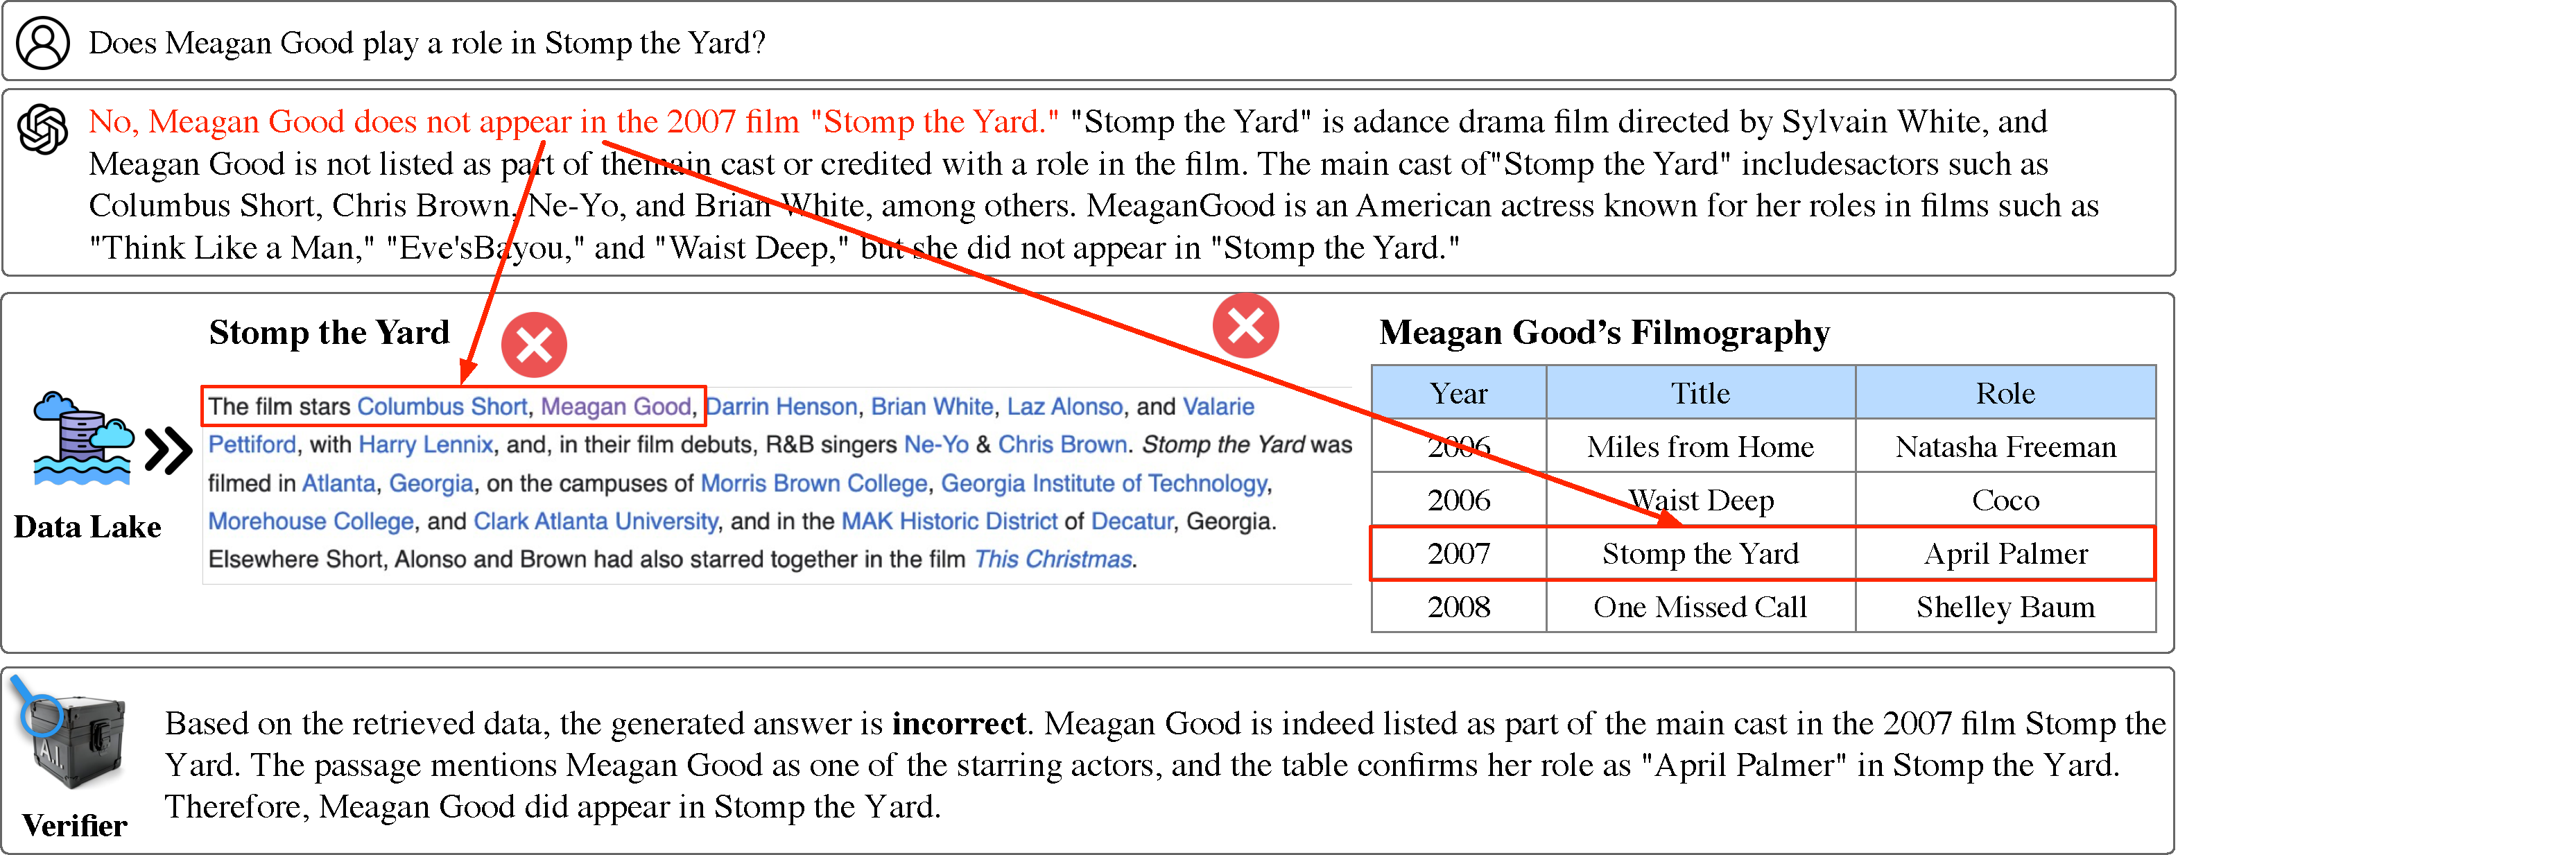
\includegraphics[width=\textwidth]{submissions/Nan2024/figs/verify.pdf}
%\vspace{-2em}
\caption{RAG-based Verification in \sys}
\label{fig:verify}
\end{center}
%\vspace{-1em}
\end{figure}
